\subsection{Solución actividad 2}
Diagrama de cuerpo libre:\\
\begin{center}
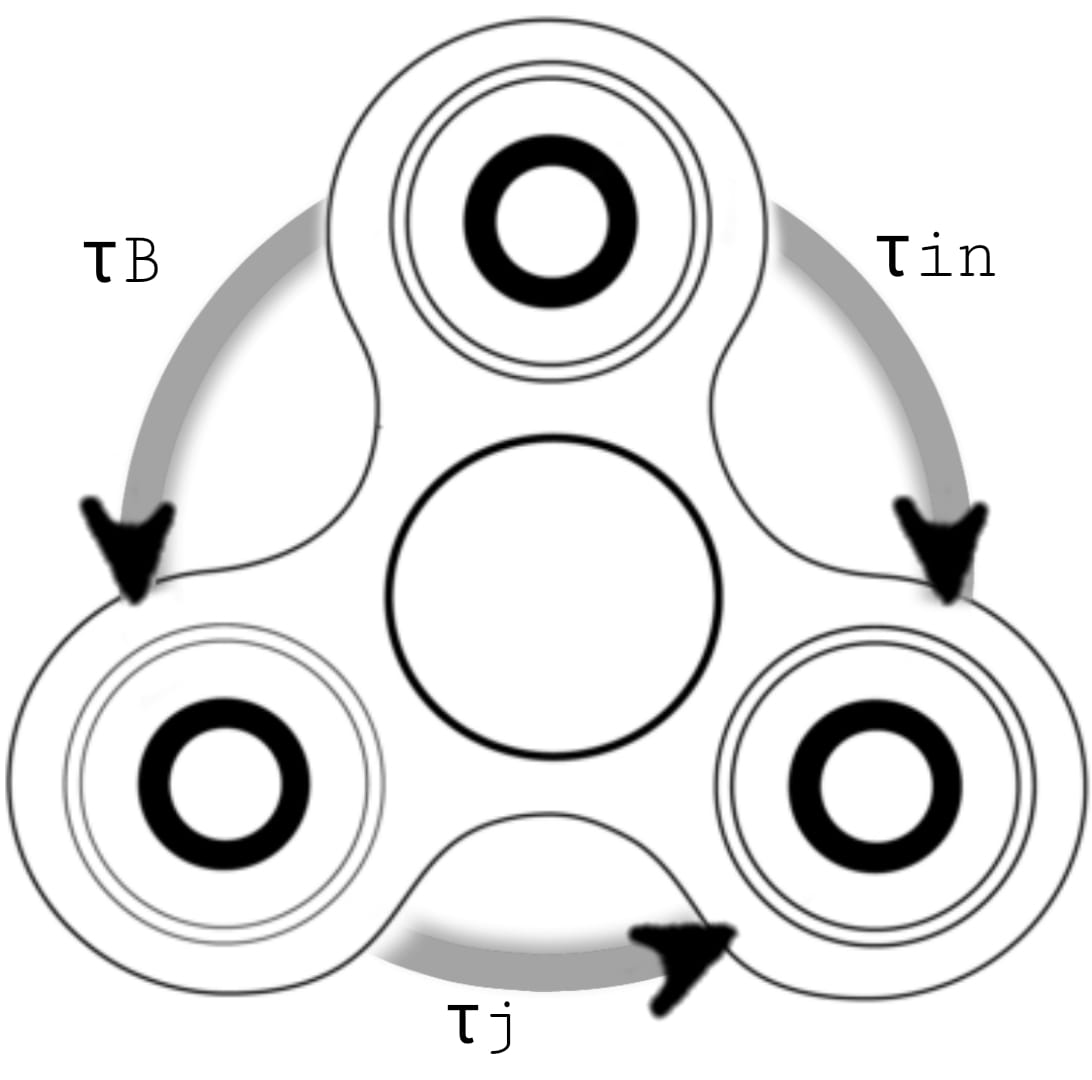
\includegraphics[scale=0.15]{DCL.jpeg} \\
\end{center}
Sistema mecánico rotacional.\\
$\tau_{in}=$Fuente de energía(Fuerza de entrada).\\
$\tau_{j}=$Masa(Inercia).\\
$\tau_{B}=$Disipador(Fricción).\\
$$\tau_{in}=\tau_{j}+\tau_{B}$$
Donde: $\tau_{j}=J\alpha,\alpha=\dot{\omega}$ y $\tau_{B}=B\omega$\\
$\alpha=\dot{\omega}=$primera derivada de la posición angular.
$$\tau_{in}=J\dot{\omega}+B\omega$$
$$\tau_{in}=J\ddot{\theta}+B\dot{\theta}$$
\textbf{Modelo matemático del sistema: $\tau_{in}=J\ddot{\theta}+B\dot{\theta}$}\\

\begin{center}
	\csvautotabular{latex/tabla.csv}
\end{center}

\subsection{Solución actividad 3}

Diagrama eléctrico equivalente:\\
\begin{center}
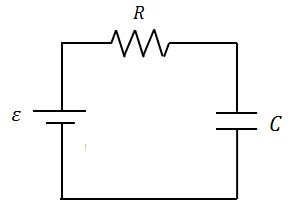
\includegraphics[scale=0.7]{ACT3.png} 
\end{center}
Donde: Capacitor(C)=masa=$\tau_{j}$, Resistencia(R)=disipador=$\tau_{B}$, Fuente de energía($\epsilon$)=$\tau_{in}$.


